\section{Introduction}
\label{sec:intro}

Recent measurements of the inclusive forward-backward $t\bar{t}$ production 
asymmetry ($A_{FB}$) from the 
Tevatron experiments show deviations from the standard model 
(SM) expectations~\cite{d0:fwtop, cdf:fwtop1, cdf:fwtop2}.
% The largest (3$\sigma$) deviation~\cite{cdf:fwtop2} is found 
% to be in the region of high invariant mass with $M_{t\bar{t}} >  450$ GeV. 
Several attempts have been made to explain this asymmetry~\cite{berger, Buckley, Gresham, zoltan}. 
One of the most natural ways to induce such an asymmetry would be through
Flavor Changing Neutral Currents (FCNC) in the top quark sector. 
The forward-backward asymmetry in $u\bar{u} \to t\bar{t}$ would then be generated
by t-channel exchange of a new massive $Z'$ boson that couples chirally to
$u$ and $t$ at the same vertex, as shown in Fig.~\ref{fig:ttbar}~\cite{berger}.
The same type of interaction would also give rise to same-sign top pair production, 
see Fig.~\ref{fig:tchannel} and Fig.~\ref{fig:schannel}. 
% Several extenstions of the SM can generate these couplings at tree level~\cite{hills, others1}.
In this case, the initial state involves two $u-$quarks and 
thus the cross section at the LHC is enhanced due 
to the large valence quark parton density of the proton. 

\begin{figure}[htb]
\begin{center}
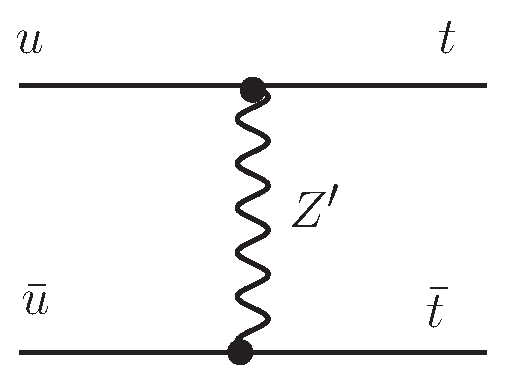
\includegraphics[width=0.35\linewidth, height=0.25\linewidth]{figs/ttbar_Z.pdf}
\caption{ Diagram for $t\bar{t}$ production induced by $Z'$ exchange which
can generate a forward-backward asymmetry. \label{fig:ttbar}}
\end{center}
\end{figure}

\begin{figure}[htb]
\begin{center}
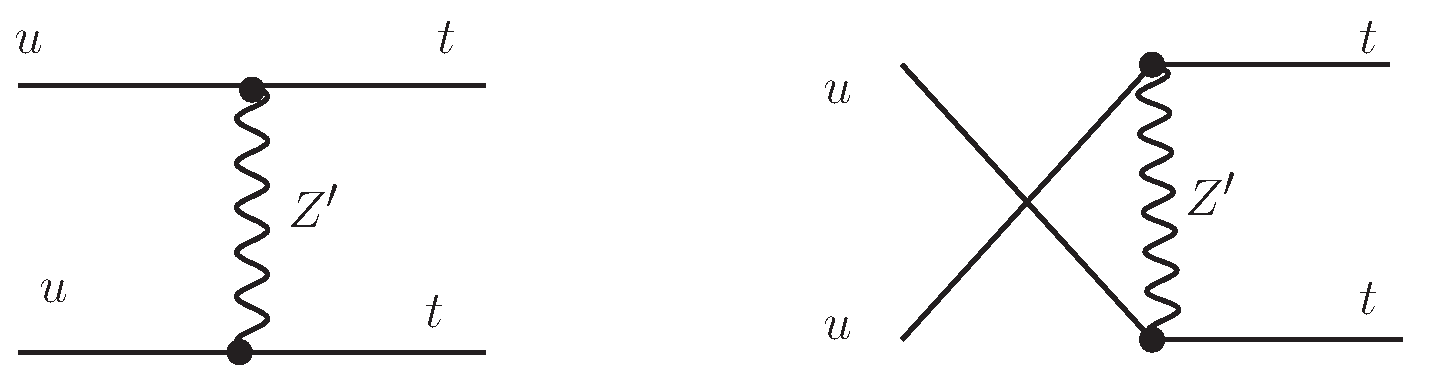
\includegraphics[width=0.7\linewidth, height=0.2\linewidth]{figs/sstop1.pdf}
\caption{ Diagrams for $tt$ pair production induced by $Z'$ exchange in the t-channel. 
\label{fig:tchannel}}
\end{center}
\end{figure}

\begin{figure}[htb]
\begin{center}
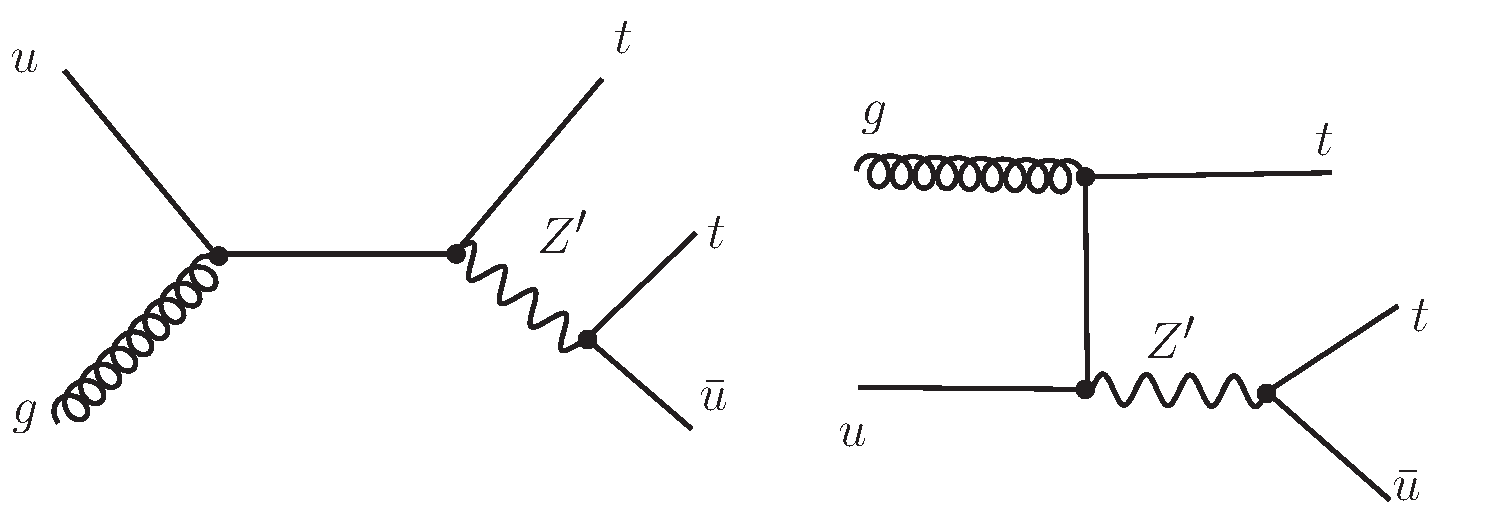
\includegraphics[width=0.7\linewidth, height=0.25\linewidth]{figs/sstop2.pdf}
\caption{ Diagrams for $tt\bar{u}$ production induced by $Z'$ exchange in the s-channel 
\label{fig:schannel}}
\end{center}
\end{figure}


%At the LHC, FCNC processes such as $uu \rightarrow tt$ can be produced via the exchange of a $Z'$ boson, 
%and can appear naturally in Techicolor (TC2) models or in general theories with non-universal massive neutral vector bosons. 
%In these models the heavy boson couples strongly to the third generation of quarks, inducing FCNC. 
%An enhancement of same-sign top pair production at the LHC via the exchange of a $Z'$ boson is predicted
%by a very recent study of the forward-backward asymmetry ~\cite{berger}.
%This detailed study also provides an explanation of the observed asymmetry at the Tevatron. 

In this work we consider the model of Reference~\cite{berger}.  
The relevant $u-t-Z'$ interaction term in the Lagrangian is:

\begin{equation}
  \mathcal{L} = g_W \bar{u} \gamma^\mu (f_L P_L + f_R P_R)tZ'_\mu + h.c
\end{equation}

where $g_W$ is the weak coupling strength. The left-handed coupling is set to $f_L = 0$, due 
to the $B_d-\bar{B_d}$ mixing constraint~\cite{Cao}. 
The right-handed coupling $f_R$ and the $Z'$ mass are free parameters in the model.
Within this model, there exists a narrow range of parameter space
consistent with the TeVatron measurements of $\sigma(p\bar{p} \to t\bar{t})$ 
and $A_{FB}$,
and not excluded by direct searches for same sign tops, see
Fig.~\ref{fig:berger_limit}.

 
% Fig.~\ref{fig:tchannel} shows the t-channel exchange diagrams that can lead to the same-sign $tt$ final state. 
% As expected the coupling appears twice in the Feynman diagrams, thus the predicated rate is proportional to $f_R^4$. 


\begin{figure}[htb]
\begin{center}
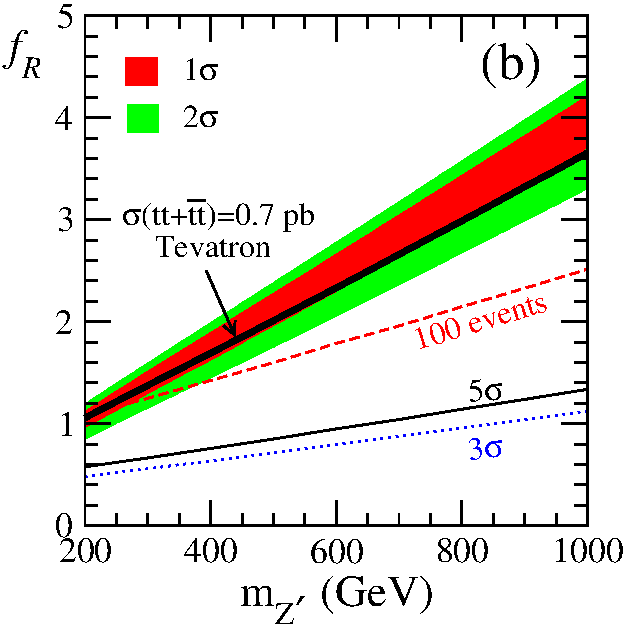
\includegraphics[width=0.6\linewidth]{figs/berger_limit.pdf}
\caption{\protect From Reference~\cite{berger}; the shaded area covers the parameter
space consistent with the $A_{FB}$ and $\sigma(t\bar{t})$ from the Tevatron;
The line indicated by the arrow shows the Tevatron limit inferred by the authors
from same sign top searches at the Tevatron; the remaining lines represent the
expectations of Reference~\cite{berger}
for LHC searches in 1 fb$^{-1}$. \label{fig:berger_limit}}
\end{center}
\end{figure}




In this study we search for same-sign di-leptons originating from $tt$ 
or $ttj$ pair production as described above.
%in the $W^+ b W^+ b$ final states, where $W^+ \rightarrow l^+ \nu$. 
To do this we exploit the approved CMS results on same sign di-leptons documented in~\cite{ssnote1, sspaper}.

This note is organized as follows: 
the signal Monte Carlo generation is described in Section~\ref{sec:mc};
in Section~\ref{sec:samesign} we give an overview of the method and results of Reference \cite{sspaper}
and we explain how these can be re-interpreted to set a limit on same-sign top production.
In Section~\ref{sec:ssresults} we present the exclusion limit derived 
as a function of the mass and coupling of the $Z'$ boson.
Finally, in Section~\ref{sec:conclusion} we summarize the results.  



% The s-channel production mode, in which the same-sign $tt$ pair is produced in association with a jet is shown in Fig.~\ref{fig:schannel}. 
% The invarient mass of the $Z'$ can be recontructed using top quarks decay modes with an additional jet in the final state. 
% As one of the initial parton is gluon initiated, we expect this rate to be lower than the t-channel diagram. 



